\documentclass{article}
\usepackage[utf8]{inputenc}
\usepackage[top=3cm, bottom=3cm, left=3cm,right=3cm]{geometry}
%\usepackage[numbers,round]{natbib}
\usepackage{natbib}
\setcitestyle{aysep={}} 
\usepackage{graphicx}
\usepackage{color}
\usepackage{amsfonts, amsmath}
\usepackage{setspace}
\usepackage{amsmath}
\usepackage{mathtools}
\usepackage{bbm}
\usepackage{float}
\usepackage{hyperref}
\usepackage[super]{nth}

\parindent0cm
\parskip0.5cm
\hyphenpenalty=10000
\pretolerance=10000
\usepackage{lineno}

% Line numbering works around align environment without requiring paragraph break
\let\oldalign\align
\let\oldendalign\endalign
\renewenvironment{align}{\linenomathNonumbers\oldalign}{\oldendalign\endlinenomath}

\linenumbers

\makeatletter
\newcommand{\customlabel}[2]{
\protected@write \@auxout {}{\string \newlabel {#1}{{#2}{}}}}
\makeatother

%\renewcommand\footnote[2][]{\relax}

\begin{document}
{\Large The epidemic lambda-coalescent model}

%Journal target:  Journal of Theoretical Biology? Theoretical Population Biology?

\vspace*{2cm}
Xavier Didelot$^{1,2,*}$, Ian Roberts$^{2}$, ...

\vspace*{2cm}
$^1$ School of Life Sciences, University of Warwick, United Kingdom\\\\
$^2$ Department of Statistics, University of Warwick, United Kingdom\\\\
$^*$ Corresponding author. Tel: 0044 (0)2476 572827. Email: \verb+xavier.didelot@gmail.com+

\vspace*{2cm}
Running title: Epidemic lambda-coalescent

\vspace*{2cm}
Keywords: lambda-coalescent model; pathogen phylogenetics; multiple mergers; offspring distribution

%\newpage
%\section*{Abstract}
%TODO

\newpage
\section{Introduction}

Superspreading in infectious disease epidemiology \citep{Lloyd-Smith2005}.
For example SARS-CoV-2 superspreading \citep{Wang2020,lemieuxPhylogeneticAnalysisSARSCoV22021,gomez-carballaSuperspreadingEmergenceCOVID192021}.
Coalescent model \citep{Kingman1982,Kingman1982a}.
Work by Li and Fraser \citep{Li2017,Fraser2017}.
Lambda-coalescent models \citep{pitmanCoalescentsMultipleCollisions1999,sagitovGeneralCoalescentAsynchronous1999,donnellyParticleRepresentationsMeasureValued1999}. 
Beta-coalescent \citep{schweinsbergCoalescentProcessesObtained2003} is a specific type of Lambda-coalescent. 
Was used in \citep{Hoscheit2019} and \citep{Menardo2021}. 
David's paper on inference of multiple mergers while dating a pathogen phylogeny \citep{Helekal2024}.

\section{General case}

Discrete time $t$. Non-overlapping generations of infected individuals. At time $t$ there are $N_t$ infected individuals. Each of them creates a number $s_{t,i}$ of secondary infections at time $t+1$, following the offspring distribution $\alpha_t(s)$. The mean of this distribution is the basic reproduction number $R_t$ and the variance is $V_t$. We have:

\begin{equation}
N_{t+1}=\sum_{i=1}^{N_t} s_{t,i}
\label{eq:summation}
\end{equation}

Let $p_{k,t}$ be the probability that $k$ individuals at time $t+1$ have the same infector at time $t$.

\subsection{Inclusive coalescence probability}

Inclusive coalescence probability $p_{k,t}(N_t, N_{t+1})$ is the probability that exactly $k$ randomly-sampled individuals from generation $t+1$ find a common ancestor in generation $t$ {\it (conditioning on population sizes $N_t$ and $N_{t+1}$.}

Given full information about offspring counts from individuals in generation $t$ ${\bf s}_t = (s_{t,1}, \dots s_{t, N_t})$, we have

{\allowdisplaybreaks
	\begin{align}
		p_{k,t}({\bf s}_t, N_t)
			& = \sum_{i=1}^{N_t} \frac{\binom{s_{t,i}}{k}}{\binom{N_{t+1}}{k}} \nonumber\\
%			& = \sum_{i=1}^{N_t} \frac{s_{t,i}!}{(s_{t,i}-k)!} \frac{(N_{t+1}-k)!}{N_{t+1}!} \\
			& = \sum_{i=1}^{N_t} \frac{\Gamma(s_{t,i}+1) \Gamma(N_{t+1}-k+1)}{\Gamma(s_{t,i}-k+1) \Gamma(N_{t+1})}.% \\
%			& = \sum_{i=1}^{N_t} \frac{s_{t,i} (s_{t,i} - 1) \dots (s_{t,i} - k + 1)}{N_{t+1} (N_{t+1} - 1) \dots (N_{t+1} - k+1)}.
	\end{align}
}

Full information $\{s_{t,i}\}$ yields the population size $N_{t+1}$ but is not feasible to observe in practice.
We can instead express the inclusive coalescence probability conditioning on the next population size $N_{t+1}$ by summing over possible offspring counts ${\bf s}_t = (s_{t,1}, \dots s_{t, N_t})$ conditional on the total generation size

{\color{red}
	To-do/To-discuss:
	\begin{itemize}
		\item Almost certainly should be an appendix not a main-body derivation, doesn't fundamentally change anything but I think this looks horrific
		\item Sum subscripts over ${\bf s}_t \in \mathbb{N}_0^{N_t}$ rather than ${\bf s}_t : ...$ (c.f. exclusive probability derivation)? We have probability 0 if sum does not equal $N_{t+1}$ anyway
		\item Change ${\bf s}_t \mapsto {\bf s}$ and $s_{t,i} \mapsto s_i$ for clarity/brevity? Should maintain $S_{t,i}$ etc. for consistent notation ($S_{t,i} = s_i$ etc.)
		\item Define $S_t^{-(1)} = (S_{t,2}, \dots, S_{t, N_t})$ notation
	\end{itemize}
}

{\allowdisplaybreaks
	\begin{align}
	p_{k,t}(N_t, N_{t+1})
		& = \sum_{{\bf s}_t : \sum_{i=1}^{N_t} s_{i,t} = N_{t+1}} \mathbb{P} \bigg[{\bf S}_t = {\bf s}_t \bigg| \sum_{i=1}^{N_t} S_{t,i} = N_{t+1} \bigg] p_{k,t}({\bf s}_t, N_t) \nonumber\\
		& = \sum_{{\bf s}_t : \sum_{i=1}^{N_t} s_{i,t} = N_{t+1}} \mathbb{P} \bigg[{\bf S}_t = {\bf s}_t \bigg| \sum_{i=1}^{N_t} S_{t,i} = N_{t+1} \bigg] \sum_{i=1}^{N_t} \frac{\binom{s_{t,i}}{k}}{\binom{N_{t+1}}{k}} \nonumber\\
		& = \sum_{i=1}^{N_t} \sum_{{\bf s}_t : \sum_{i=1}^{N_t} s_{i,t} = N_{t+1}} \frac{\binom{s_{t,i}}{k}}{\binom{N_{t+1}}{k}} \mathbb{P} \bigg[S_{t,1} = s_{t,1}, {\bf S}_t^{-(1)} = {\bf s}_t^{-(1)} \bigg| \sum_{i=1}^{N_t} S_{t,i} = N_{t+1} \bigg] \nonumber\\
		& = \frac{N_t}{\binom{N_{t+1}}{k}} \sum_{{\bf s}_t : \sum_{i=1}^{N_t} s_{i,t} = N_{t+1}} \binom{s_{t,1}}{k} \mathbb{P} \bigg[S_{t,1} = s_{t,1} \bigg| \sum_{i=1}^{N_t} S_{t,i} = N_{t+1} \bigg] \nonumber \\
			& \phantom{=}\qquad \times \mathbb{P} \bigg[{\bf S}_t^{-(1)} = {\bf s}_t^{-(1)} \bigg| S_{t,1} = s_{t,1}, \sum_{i=1}^{N_t} S_{t,i} = N_{t+1} \bigg] \nonumber\\
		& = \frac{N_t}{\binom{N_{t+1}}{k}} \sum_{s_{t,1} = 0}^{N_{t+1}} \binom{s_{t,1}}{k} \mathbb{P} \bigg[S_{t,1} = s_{t,1} \bigg| \sum_{i=1}^{N_t} S_{t,i} = N_{t+1} \bigg] \nonumber \\
			& \phantom{=}\qquad \times \underbrace{\sum_{{\bf s}_t^{-(1)} : \sum_{i=2}^{N_t} s_{i,t} = N_{t+1} - s_{1,t}} \mathbb{P} \bigg[{\bf S}_t^{-(1)} = {\bf s}_t^{-(1)} \bigg| \sum_{i=2}^{N_t} S_{t,i} = N_{t+1} - s_{1,t} \bigg]}_{=1} \nonumber\\
		& = \frac{N_t}{\binom{N_{t+1}}{k}} \mathbb{E}\bigg[ \binom{S_{t,1}}{k} \bigg| \sum_{i=1}^{N_t} S_{t,i} = N_{t+1} \bigg] \label{eq:GeneralInclusiveProb} %\nonumber\\
%		& = N_t \frac{(N_{t+1} - k)!}{N_{t+1}!} \mathbb{E} \bigg[ \frac{S_{t,1}!}{(S_{t,1} - k)!} \bigg | \sum_{i=1}^{N_t} S_{t,i} = N_{t+1} \bigg]. \label{eq:GeneralInclusiveProb}
	\end{align}
}

The falling factorial moments $\mathbb{E} \big[ \frac{S_{t,1}!}{(S_{t,1} - k)!} \big | \sum_{i=1}^{N_t} S_{t,i} = N_{t+1} \big]$ in \eqref{eq:GeneralInclusiveProb} can be readily obtained by differentiating the probability generating function of $S_{t,1} | (\sum_{i=1}^{N_t} S_{t,i} = N_{t+1})$.

\subsection{Exclusive coalescence probability}

Generally, we observe a sample of individuals from each generation rather than the entire population.
In this case, we are interested in the exclusive coalescence probability $p_{nkt}(N_t, N_{t+1})$ that exactly $k$ individuals from a sample of $n$ arose from a common ancestor one generation in the past given knowlege of the total population sizes $N_t$ and $N_{t+1}$.

Given full information about offspring counts of the parents of sampled individuals at the present, ${\bf x}_t = (x_{t,1}, \dots, x_{t,N_t})$, we have
	\begin{align}
		p_{nkt}({\bf x}_t, N_t)
			& = \sum_{i=1}^{N_t} \frac{\binom{x_{t,i}}{k}}{\binom{n}{k}} \mathbb{I} \{ x_{t,i} = k \}\nonumber\\
			& = \sum_{i=1}^{N_t} \frac{x_{t,i}!}{(x_{t,i} - k)!} \frac{(n-k)!}{n!} \mathbb{I} \{ x_{t,i} = k \}.
	\end{align}

Similarly to the exclusive coalescence probability, we can use this to evaluate the exclusive probability given $N_t$ and $N_{t+1}$ by summing over possible parent offspring configurations (for $k \leq n$),

{\allowdisplaybreaks
	\begin{align}
		p_{nkt}(N_t, N_{t+1})
			& = \sum_{{\bf x}_t \in \mathbb{N}_0^{N_t}} \mathbb{P} \bigg[ {\bf X}_t = {\bf x}_t \bigg | \sum_{i=1}^{n} X_{t,i} = n \bigg] p_{n,k,t} ({\bf x}_t, N_t) \nonumber\\
			& = \sum_{{\bf x}_t \in \mathbb{N}_0^{N_t}} \mathbb{P} \bigg[ {\bf X}_t = {\bf x}_t \bigg | \sum_{i=1}^{n} X_{t,i} = n \bigg] \sum_{i=1}^{N_t} \frac{\binom{x_{t,i}}{k}}{\binom{n}{k}} \mathbb{I} \{ x_{t,i} = k \} \nonumber\\
			& = \frac{N_t}{\binom{n}{k}} \sum_{{\bf x}_t \in \mathbb{N}_0^{N_t}} \binom{x_{t,1}}{k} \mathbb{P} \bigg[ {\bf X}_t = {\bf x}_t \bigg| \sum_{i=1}^{N_t} X_{t,i} = n \bigg] \mathbb{I} \{x_{t,1} = k \} \nonumber\\
			& = \frac{N_t}{\binom{n}{k}} \sum_{{\bf x}_t^{-(1)} : \sum_{i=2}^n x_{t,i} = n-k} \binom{k}{k} \mathbb{P}\bigg[X_{t,1} = k, {\bf X}_t^{-(1)} = {\bf x}_t^{-(1)} \bigg| \sum_{i=1}^{N_t} X_{t,i} = n \bigg] \nonumber\\
			& = \frac{N_t}{\binom{n}{k}} \mathbb{P}[X_{t,1} = k \bigg| \sum_{i=1}^{N_t} X_{t,i} = n \bigg] \sum_{{\bf x}_t^{-(1)} : \sum_{i=2}^n x_{t,i} = n-k} \mathbb{P}\bigg[{\bf X}_t^{-(1)} = {\bf x}_t^{-(1)} \bigg| \sum_{i=1}^{N_t} X_{t,i} = n, X_{t,1} = k \bigg] \nonumber\\
			& = \frac{N_t}{\binom{n}{k}} \mathbb{P} \bigg[ X_{t,1} = k \bigg| \sum_{i=1}^{N_t} X_{i,t} = n \bigg]. \label{eq:GeneralExclusiveProb}
	\end{align}
}

\subsection{Complementarity of exclusive coalescence probabilities}

Note that for any offspring distribution we have:

\begin{equation}
\sum_{k=1}^n p_{nkt} \binom{n-1}{k-1}=1
\end{equation}

	\begin{align}
		\sum_{k=1}^n \binom{n-1}{k-1} p_{nkt}
			& = \sum_{k=1}^n \binom{n-1}{k-1} \frac{N_t}{\binom{n}{k}} \mathbb{P}[X_1 = k | \sum_{i=1}^{N_t} X_i = n] \\
			& = \sum_{k=1}^n N_t \frac{k}{n} \mathbb{P}[X_1=k | \sum_{i=1}^{N_t} X_i = n] \\
			& = \frac{N_t}{n} \sum_{k=0}^n k \mathbb{P}[X_1 = k | \sum_{i=1}^{N_t} X_i = n] \tag{lower limit $k=0$ makes no difference overall}\\
			& = \frac{N_t}{n} \mathbb{E}[X_1 | \sum_{i=1}^{N_t} X_i = n ] \\
			& = p_{1,t} (N_t, n) = 1 \tag{see below}
	\end{align}
	
	Taken from \href{https://math.stackexchange.com/questions/2508465/conditional-expectation-of-random-variable-given-a-sum}{stackexchange (link)}
	
	\begin{align}
		\mathbb{E}[X_1 | \sum_{i=1}^{N_t} X_i = n]
			& = \frac{1}{N_t} \sum_{i=1}^{N_t} \mathbb{E}[X_i | \sum_{i=1}^{N_t} X_i = n] \tag{$X_i$ i.i.d.} \\
			& = \frac{1}{N_t} \mathbb{E}[ \sum_{i=1}^{N_t} X_i | \sum_{i=1}^{N_t} X_i = n] \tag{Swap expectation, sum \it (possibly questionable?)} \\
			& = \frac{n}{N_t}
	\end{align}
	
\section{Poisson case}

Here the offspring distribution is $\alpha_t = \text{Poisson}(R_t)$.
In this case, we have 
	\begin{equation}
		\sum_{i=1}^{N_t} S_{t,i} \sim \text{Poisson}(N_t R_t),
	\end{equation}
and conditional distribution
{\allowdisplaybreaks
	\begin{align}
		\mathbb{P}\bigg[S_{t,1} = s \bigg| \sum_{i=1}^{N_t} S_{t,i} = N_{t+1} \bigg]
			& = \frac{\displaystyle\mathbb{P}\bigg[S_{t,1} = s, \sum_{i=1}^{N_t} S_{t,i} = N_{t+1} \bigg]}{\displaystyle\mathbb{P}\bigg[\sum_{i=1}^{N_t} S_{t,i} = N_{t+1} \bigg]} \\
			& = \frac{\displaystyle\alpha_t (s) \, \mathbb{P}\bigg[ \sum_{i=2}^{N_t} S_{t,i} = N_{t+1} - s \bigg]}{\displaystyle\mathbb{P}\bigg[\sum_{i=1}^{N_t} S_{t,i} = N_{t+1} \bigg]} \\
			& = \frac{\displaystyle\frac{R_t^s e^{-R_t}}{s!} \cdot \frac{((N_t - 1)R_t)^{N_{t+1} - s}}{(N_{t+1} - s)!}}{\displaystyle\frac{(N_t R_t)^{N_{t+1}} e^{-N_t R_t}}{N_{t+1}!}} \\
			& = \binom{N_{t+1}}{s} \left( \frac{1}{N_t} \right)^s \left( 1 - \frac{1}{N_t} \right)^{N_{t+1} - s}, 
	\end{align}
}
that is
	\begin{equation}
		S_{t,1} \bigg| \left(\sum_{i=1}^{N_t} S_{t,i} = N_{t+1}\right) \sim \text{Binomial}\left(N_{t+1}, \frac{1}{N_t}\right).
	\end{equation}

The inclusive probability of coalescence for $k$ lines is given by \eqref{eq:GeneralInclusiveProb} with the falling factorial moments
\begin{equation}
	\mathbb{E} \left[ \binom{S_{t,1}}{k} \bigg| \sum_{i=1}^{N_t} S_{t,i} = N_{t+1} \right]
		= \frac{1}{k!} \mathbb{E} \left[ \frac{S_{t,1}!}{(S_{t,1} - k)!} \bigg| \sum_{i=1}^{N_t} S_{t,i} = N_{t+1} \right]
		= \frac{1}{k!} \, \frac{N_{t+1}!}{(N_{t+1} - k)!} \left( \frac{1}{N_t} \right)^k,
\end{equation}
taken from \cite{Potts1953}.

Consequently, the inclusive probability of coalescence for two lines is
\begin{equation}
	p_{2,t}=\frac{1}{N_t},
\end{equation}
and more generally the inclusive probability of coalescence for $k$ lines is
\begin{equation}
	p_{k,t}=\frac{1}{N_t^{k-1}}.
\end{equation}
The inclusive probability of coalescence for two lines is analogous to the Wright-Fisher model, with each individual at generation $t+1$ selecting a parent uniformly at random from generation $t$.



The exclusive probability of coalescence for two lines from a sample of $n$ $(n \geq 2)$ is
	\begin{equation}
		p_{n,2,t} = \frac{(N_t-1)^{n-2}}{N_t^{n-1}},
	\end{equation}
and more generally the exclusive probability of coalescence for $k$ lines from a sample of $n$ $(n \geq k)$ is
	\begin{equation}
		p_{n,k,t} = \frac{(N_t-1)^{n-k}}{N_t^{n-1}}.
	\end{equation}

\section{Negative-Binomial case}

Here the offspring distribution is Negative-Binomial with mean $R_t$ and variance $V_t$.
The parameters of this distribution are 
$r=R_t^2/(V_t-R_t)$ and $p=R_t/V_t$.

The inclusive probability of coalescence for two lines is:

\begin{equation}
p_{2,t}=\frac{r+1}{N_t r+1}
\end{equation}

The inclusive probability of coalescence for $k$ lines is:

\begin{equation}
p_{k,t}=\prod_{i=1}^{k-1}\frac{r+i}{N_t r+i}=\frac{\mathrm{B}(N_t r+1,r+k)}{\mathrm{B}(r+1,N_t r+k)}
\end{equation}

\noindent where  $\mathrm{B}(x,y)$ denotes the Beta function defined as $\mathrm{B}(x,y)=\Gamma(x)\Gamma(y)/\Gamma(x+y)$.

The exclusive probability of coalescence for $k$ lines is:

\begin{equation}
p_{nkt}=\frac{N_t \mathrm{B}(k+r, n-k+N_t r-r)}{\mathrm{B}(r, N_t r-r)}
\end{equation}

\section{Example}

Let the offspring distribution have a mean of $R_t=2$. In the Poisson case the offspring distribution is Poisson(2). We consider NegBin cases with the same mean and varying dispersion parameters $r$. When $r$ is high the dispersion is low and the NegBin behaves almost like a Poisson.
See Figure \ref{fig:probs}.

\begin{figure}[t!]
\begin{center}
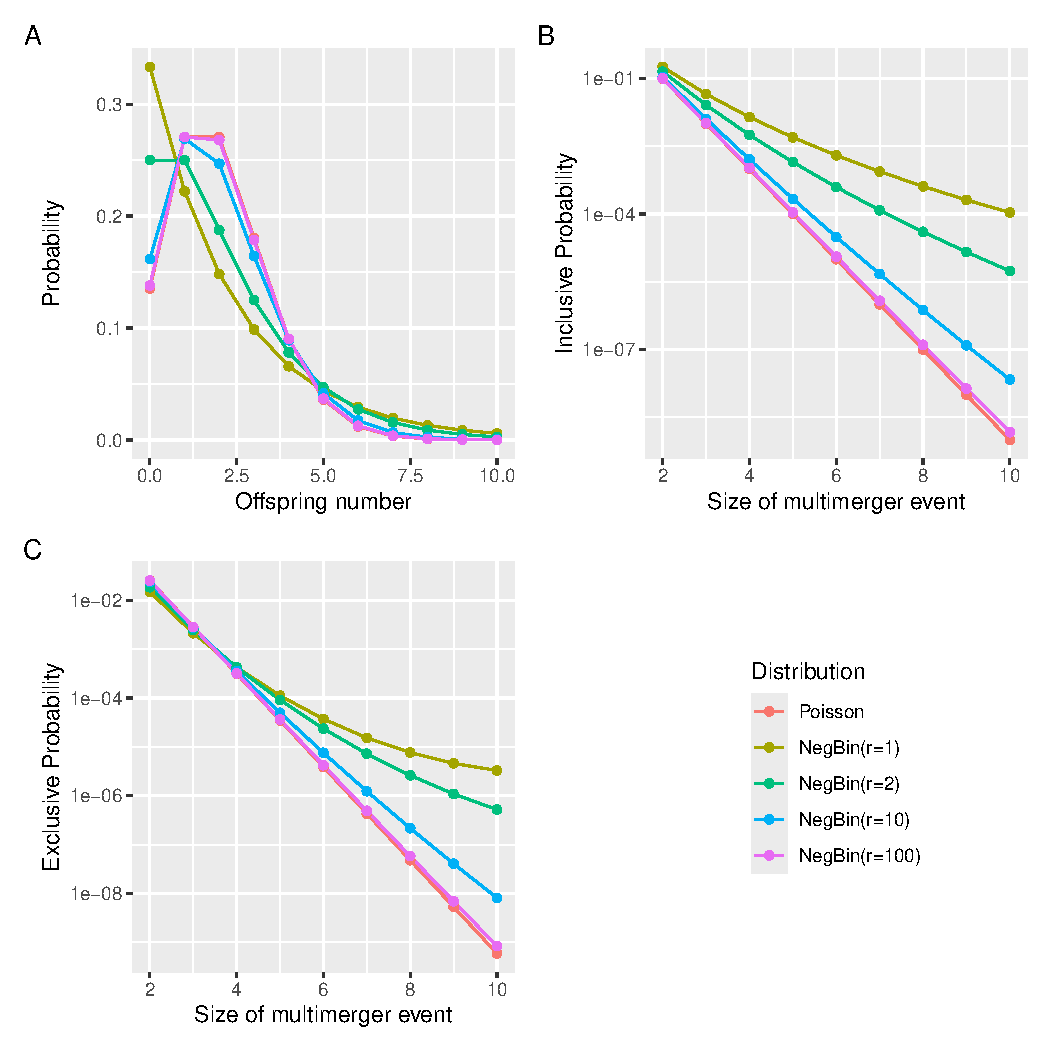
\includegraphics[width=15cm]{../run/figure.pdf}
\end{center}
\caption{(A) Offspring distribution. (B) Inclusive probability of coalescence. (C) Exclusive probability of coalescence.
\label{fig:probs}}
\end{figure}

\section{Lambda-coalescent}

A lambda-coalescent model is defined by a probability measure 
$\Lambda(\mathrm{d} x)$ on the interval $[0,1]$, from which we can deduce
the rate $\lambda_{n,k}$ at which any subset of $k$ lineages within a set of $n$ observed lineages 
coalesce:

\begin{equation}
    \lambda_{n,k} = \int_{0}^{1}{x^{k-2}(1-x)^{n-k}\,\Lambda(\mathrm{d} x)}
\end{equation}

The Beta$(2-\alpha,\alpha)$-coalescent model \citep{schweinsbergCoalescentProcessesObtained2003}
has a single parameter $\alpha \in [0,2]$ and is defined as:

\begin{equation}
\Lambda(\mathrm{d}x)=\frac{x^{1-\alpha}(1-x)^{\alpha-1}}{\mathrm{B}(2-\alpha,\alpha)}\mathrm{d}x
\end{equation}

from which we can deduce that:

\begin{equation}
\lambda_{n,k}=\frac{\mathrm{B}(k-\alpha,n-k+\alpha)}{\mathrm{B}(2-\alpha,\alpha)}
\end{equation}

Special cases include $\alpha=2$ corresponding to the Kingman coalescent,
$\alpha=1$ which is known as the Bolthausen-Sznitman coalescent
and $\alpha=0$ for which the phylogeny is always star-shaped.

\section{Implementation}

We implemented the analytical methods described in this paper in a 
new R package entitled \emph{EpiLambda} which is available
at \url{https://github.com/xavierdidelot/EpiLambda} for R version 3.5 or later. 
All code and data needed to replicate the results are included in the ``run'' directory of the \emph{EpiLambda} repository.

\section{Discussion}

\section*{Acknowledgements}

We acknowledge funding from the National Institute for Health Research (NIHR) Health Protection Research Unit in Genomics and Enabling Data.

\newpage
\bibliographystyle{elsarticle-harv}
%\bibliography{biblio,/Users/u1775021/all.bib}
\bibliography{biblio}

\end{document}

